\documentclass[conference]{IEEEtran}
\IEEEoverridecommandlockouts
\setlength{\columnsep}{6mm}
\usepackage{hyperref}
\usepackage{cite}
\usepackage{amsmath,amssymb}
\usepackage{algorithmic}
\usepackage{graphicx}
\usepackage{textcomp}
\usepackage{xcolor}
\usepackage{stfloats}
\usepackage{booktabs}
\usepackage{url}
\usepackage{algorithm}
\usepackage{multirow}
\usepackage{flushend}
\usepackage{subfigure}
\usepackage{url}

% -------- for figures --------
\usepackage{tikz,graphicx,pgfplots,tikz-layers,fontawesome5}
\usepackage{colortbl, tabto}
\pgfplotsset{compat=1.18}
\usetikzlibrary{shapes,calc,positioning,fit,decorations,decorations.text, arrows,arrows.meta}
\usepackage{amssymb,amsmath,enumitem,lipsum}
\usepackage{multirow,fancyhdr}
\usepackage{array,xcolor}
\usepackage{rotating}
% -------- end figures --------

%\usepackage{endnotes}
\usepackage{enotez}
\setenotez{list-name=References}
\let\footnote=\endnote
%\setlength{\parindent}{0pt}
\def\UrlBreaks{\do\A\do\B\do\C\do\D\do\E\do\F\do\G\do\H\do\I\do\J
	\do\K\do\L\do\M\do\N\do\O\do\P\do\Q\do\R\do\S\do\T\do\U\do\V
	\do\W\do\X\do\Y\do\Z\do\[\do\\\do\]\do\^\do\_\do\`\do\a\do\b
	\do\c\do\d\do\e\do\f\do\g\do\h\do\i\do\j\do\k\do\l\do\m\do\n
	\do\o\do\p\do\q\do\r\do\s\do\t\do\u\do\v\do\w\do\x\do\y\do\z
	\do\.\do\@\do\\\do\/\do\!\do\_\do\|\do\;\do\>\do\]\do\)\do\,
	\do\?\do\'\do+\do\=\do\#}
\makeatletter
\newcommand{\rmnum}[1]{\romannumeral #1}
\newcommand{\Rmnum}[1]{\expandafter\@slowromancap\romannumeral #1@}
\makeatother

\def\BibTeX{{\rm B\kern-.05em{\sc i\kern-.025em b}\kern-.08em
    T\kern-.1667em\lower.7ex\hbox{E}\kern-.125emX}}
\begin{document}

\title{{Omron Network - Verified Intelligence} \\

{\footnotesize}
}


\author{
\IEEEauthorblockA{{By: Colin Gagich, Ronald Chan, Spencer Graham, Will Prangley} \\
{Inference Labs Inc. - \url{inferencelabs.com}}\\
%E-mails: investor@inferencelabs.com
}
\IEEEauthorblockN{Feb 23 2024 (v1.01)}%, xyz i\IEEEauthorrefmark{1} and xyzi \IEEEauthorrefmark{1} and xyzz\IEEEauthorrefmark{1} and xyz\IEEEauthorrefmark{1}}

}
\maketitle

% change page style back to plain to enable page numbers
\thispagestyle{plain}
\pagestyle{plain}
% end of adding page numbers

\begin{abstract}
Our mission transcends merely bringing the next billion humans to web3; we aim to usher in trillions of users - be they human or machine.

`The future of AI and next level of super intelligence is not one extremely capable system but a path towards billions if not a trillion copies of capable AIs' - Sam Altman, Sept 13, 2023 

Inference Labs is extending the decentralized and verifiable world computer by embedding the capabilities of cryptographically verified, off-chain artificial intelligence within it. 
The dilemma? The surge in interest in autonomous AI agents is unparalleled. Machine internet traffic will soon outpace human activity.\endnote{Bradley, J., Barbier, J., Handler, D. (2013). Embracing the Internet of Everything To Capture Your Share of \$14.4 Trillion. Cisco. \url{https://www.cisco.com/c/dam/en_us/about/ac79/docs/innov/IoE\_Economy.pdf - Predicts that machine-to-machine traffic will be over 40\% of total IP traffic by 2022}} Web2 can't meet all of AI agents' financial needs. While blockchains suit value exchange, current ones don't accommodate AI. Running inferences off-chain risks intellectual property and forces users to compromise on trust, sovereignty, and economic risks by depending on centralized points of failure.\endnote{Turchin, A., Denkenberger, D. (2018). Classification of global catastrophic risks connected with artificial intelligence. AI Safety and Security. CRC Press. \url{https://www.crcpress.com/Artificial-Intelligence-Safety-and-Security/Yampolskiy/p/book/9780429298339 - Discusses risks of centralized control over advanced AI}.}

Over recent years, zero-knowledge cryptography has played a pivotal role in blockchain advancements for two primary reasons: (1) they enhance the scalability of compute-limited networks by handling transactions off-chain and subsequently confirming the outcomes on mainnet; and (2) they bolster user confidentiality by facilitating veiled transactions, which are only accessible to those with knowledge of the concealed details. For platforms like Ethereum, scalability can't be achieved without overburdening validators, leading to the adoption of rollups. Given the transparent nature of transactions, on-chain privacy is also essential. Beyond these, zero-knowledge cryptography ensure efficient validation of any computation, not just those linked to an off-chain EVM, revealing their broad potential beyond blockchains. The utility of zero-knowledge cryptography isn't confined to these two aspects. They also offer a third critical advantage: the efficient validation that any computation, not just those associated with an off-chain version of the EVM, has been executed accurately. This potential extends well beyond the realm of blockchains.

In this paper we present Omron Network, a decentralized protocol and network to run off-chain inference securely and verified with zero-knowledge cryptography.

\end{abstract}

%\begin{IEEEkeywords}  Blockchain; Data Sharing; SGX; Security; Privacy; Smart Contract

%\end{IEEEkeywords}

\section{Introduction}
In the current centralized model of AI governance, significant vulnerabilities exist. This model, susceptible to unauthorized changes and censorship by privileged entities, impedes the smooth transaction of value across different ecosystems and requires a reliance on trust, introducing considerable security and financial risks. Centralization conflicts with the stringent requirements of tamper-proof, trustless smart contracts, which operate independently on decentralized platforms like blockchains. They are immune to tampering, ensuring a unique trust paradigm independent of any single entity. This makes a compelling case for a shift towards a decentralized approach, enhancing the creation and management of digital agreements in a manner that is both human and machine-readable, paving the way for a more advanced and intelligent web3 era.

The advent of blockchains and their transaction-based architecture, however, brings forth the challenge of Connectivity for off-chain Neural Networks.  This issue arises from the inability of blockchains to directly engage with off-chain AI Neural Networks, which are too large and computationally intensive to reside on-chain. Additionally, the current reliance on centralized processes for inference calculations in smart contracts introduces a dependency on the operators' integrity, undermining the trust and security that smart contracts are designed to offer. AI's inherent "black box" nature further complicates matters, with its concealed biases and dynamic algorithms posing a threat to system security and user assets.

To address these challenges, we propose the Omron Network, a solution that stands out in the realm of zk-ML solutions. Omron is a secure, decentralized network that is chain interoperable and zk-proving system agnostic, ensuring the tamperproof integrity vital for smart contracts. Unlike existing solutions, Omron operates as a wholly decentralized network, reducing reliance on any single entity and guaranteeing a secure, seamless exchange of value and operations. This framework marks a significant step towards overcoming the limitations of current blockchain-AI interactions, fostering a more secure and efficient environment for the expanding web3 community.
\subsection{Rationale for AI x Web3}
Artificial intelligence represents one of the most transformative technologies of our time. However, the full benefits of AI remain restricted to large tech firms with sufficient data and resources. This centralization limits innovation and prevents many from accessing AI's immense potential.  

Web3 proposes an alternative through open and decentralized networks, aspiring to transform AI systems into publicly accessible infrastructure, thereby amplifying and sharing the economic and social benefits. However, the aspiration to run on-chain neural networks is currently hindered by the technical constraints of blockchain technology which struggles with the high demands of computational power and storage required by such models. Furthermore, there's the significant challenge of protecting the intellectual property embedded within AI models; running them on-chain will inadvertently expose proprietary algorithms and data sets. Despite these challenges the vision of democratizing AI is the same as how open source software democratized computing.

The application of cryptography primitives to AI unlocks transformative decentralized business models powered by verifiable intelligence while intellectual property remains concealed.  Web3 serves as the ideal base layer for reshaping AI systems to run securely on decentralized networks instead of within closed corporate silos.

Smart contracts have technical and practical limitations. Not every problem can be solved within 24kB of bytecode. Not every solution can be expressed as a closed form mathematical expression. Extending smart contract capabilities with heuristically derived AI models is the next logical step. Oracles are third party services which provide external data and computations to blockchain applications. The outputs from oracles must be trusted regardless if it is one or many coordinated actors.  In contrast, secure machine learning changes the paradigm with on-chain verification of AI model executions, eliminating the need for third-party trust. Such deterministic AI models, when incorporated into the blockchain, behave in a predictable and immutable manner.

This determinism and verifiability guarantees predictions from an AI model cannot be influenced or corrupted by any party. The model becomes an unbiased "oracle" once deployed and executed on-chain. Unlike traditional oracles its inferences are independently and transparently verified. \\

Examples of next-generation applications enabled by verified Artificial Intelligence:
\begin{itemize}
    \item \textbf{Decentralized Finance:}  On-chain AI models analyze market signals and optimize trading strategies in a transparent and tamper-proof manner. For example, an AI predicting asset price volatility could inform options pricing or portfolio rebalancing. And decentralized lending protocols may rely on verified AI credit risk models for loan approvals.
    \item \textbf{Security and Compliance:} By monitoring for atypical transaction patterns, AI will aid in preemptive threat identification and bolster risk management. Large Language Models (LLMs) will translate human language instructions into code for smart contract auditing.
    \item \textbf{Identity Verification:} A verified AI system will play a pivotal role in "Proof-of-Personhood" validations, ensuring one vote per verified human in decentralized governance systems without compromising anonymity and integrity.
    \item \textbf{Gaming Ecosystems:} AI will be used to coordinate AI vs. AI matches, manage in-game economics, and verify the integrity of games to prevent cheating and ensure fair play for all participants.
\end{itemize}

\subsection{Rationale for Model Privacy}
Proprietary machine learning models represent the core intellectual property for organizations. These models are often developed over countless hours and substantial investment. They incorporate unique weights and biases which directly contribute to their performance, accuracy, and competitive advantage. Protecting the confidentiality of these assets is crucial not only to preserve the commercial value but also to maintain the integrity and reputation of the models themselves.\endnote{Yousef, A. J., \& Allam, A. (2018). Privacy-Preserving Machine Learning: Threats and Solutions. IEEE Security \& Privacy, 16(2), 49–58. https://doi.org/10.1109/MSP.2018.2701156}

Open access to the intricacies of a model such as its training methods, fine-tuning processes, and the data on which it was trained—could enable third parties to replicate and potentially misuse the technology. Such replication might not only violate intellectual property rights but also lead to versions of the model which do not uphold the standards, values, or performance metrics set by the original creators. Misuse or misrepresentation of AI capabilities, sometimes referred to as "pseudo-AI," can erode trust in the technology and its providers, casting a shadow over legitimate and ethically developed AI services.

\textbf{Use Case: Proprietary Trading Algorithms}

In the financial sector, proprietary trading algorithms are developed using ML to predict market movements and automate trading decisions. These algorithms are trained on historical data, real-time market feeds, and a myriad of other quantitative inputs. The model weights and biases are fine-tuned to identify patterns in market trends.

If the details of these algorithms were made public, it could lead to several negative outcomes:

If the strategy is effective, competitors will replicate the trading strategy hereby saturating the market signals, thus diluting its effectiveness.

Malicious actors will design strategies specifically to exploit the known behaviors of the publicized algorithm or otherwise front-run it.

The financial institution could lose its unique market positioning, which is built on the strength and secrecy of its trading strategies.

To protect the integrity, effectiveness, and commercial value of these algorithms it is essential for creators to keep their weights and biases confidential. In doing so, they not only preserve their competitive advantage but also the security and commercial viability of their intellectual property.
\subsection{Rationale for Model Authenticity}
AI models are already making decisions in cases where humans, especially on the level of the individual, are likely to have inherent bias. The decisions of judges and juries are often studied and many factors irrelevant to a case consciously and subconsciously have an effect. Such factors include but are not limited to the appearance, race, and history of the defendant, or the personal history of the judge.\endnote{\url{https://scholarship.law.cornell.edu/cgi/viewcontent.cgi?article=1691&context=facpub}} Countries such as Malaysia and Estonia have pilot programs which use AI to determine sentencing lengths and mediate disputes between parties.\endnote{\url{https://www.reuters.com/article/malaysia-tech-lawmaking-idUSL8N2HD3V7}}\endnote{\url{https://www.wired.com/story/can-ai-be-fair-judge-court-estonia-thinks-so/}}   

The creation of a fair AI judgment system is a challenge all on its own; an AI system built by humans will likely contain the same biases due to its training data and validation techniques.\endnote{\url{https://www.vox.com/future-perfect/22916602/ai-bias-fairness-tradeoffs-artificial-intelligence}}  However, one promise is the consistency and objectivity of an AI algorithm. Once a bias is found the impact of changes made can be measured and further optimized to show a reduction in bias.\endnote{\url{https://itif.org/publications/2020/01/27/critics-were-wrong-nist-data-shows-best-facial-recognition-algorithms/}} A system which repeatedly delivers the same result may be preferable over one in which the time of day and proximity to lunchtime has an effect on the chance of parole.\endnote{\url{https://www.ncbi.nlm.nih.gov/pmc/articles/PMC3198355/}}

With all this considered, society may one day have an AI model which is considered fair and is agreed upon as the standard for determining sentences. This leads to the next issue, who runs the AI model and how does one know it was run correctly? It is self-evident all parties involved in the process want certainty in the algorithm's correct execution.

\subsection{Preliminary on AI Neural Networks}
Neural networks, often referred to as artificial neural networks (ANNs) or simulated neural networks (SNNs), are central to deep learning, a pivotal component of machine learning. Their design, reminiscent of the human brain, emulates the intricate signaling between biological neurons. ANNs consist of layered nodes, which include an input layer, several hidden layers, and an output layer. Each node connects to others, possessing a distinct weight and threshold. A node becomes active and transmits data to the subsequent layer only if its output surpasses its threshold; otherwise, it remains dormant.

The efficacy of neural networks hinges on extensive training data, allowing them to refine their accuracy progressively. When optimized, these algorithms stand as formidable pillars in computer science and AI, enabling swift data classification and clustering. Such efficiency transforms tasks like speech and image recognition, reducing tasks that might take humans hours into mere minutes.

Each node in a neural network represents a miniature linear regression model, with its own inputs, weights, bias, and output. Simplistically the formula is: \\

$w_i = $ \text{weight for }$i'th$\text{ element}

$x_i = $  $i'th$ element

$b = bias$

$$\begin{aligned} & 
\sum w_{\mathrm{i}} x_{\mathrm{i}}+b=w_1 x_1+w_2 x_2+w_3 x_3+b \\ &
\text { output }=f(x)=1 \text { if } \sum w_{\mathrm{i}} x_{\mathrm{i}}+b>=0 ; \\ 
& 0 \text { if } \sum w_{\mathrm{i}} x_{\mathrm{i}}+b<0\end{aligned}$$

\begin{figure}[!ht]
    \centering
    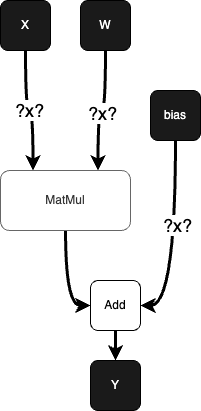
\includegraphics[width=0.18\textwidth]{figures/ai-model-matmul.png}
    \caption{Example MatMul and Bias Computational Graph}
    \label{fig:Fig 2}
\end{figure}

An activation function is applied, outputting 1 if the result is non-negative and 0 otherwise. Once data enters the network, weights are allocated to different inputs. These weights highlight the significance of each input, with larger weights implying a greater influence on the output. Inputs are weighted, summed, and processed through the activation function. If the resulting output surpasses a particular threshold, the node activates and sends data to the subsequent layer. This flow of information from one layer to another typifies a feedforward network.

\noindent The following is Not Financial Advice (NFA)

As a simple example with binary representation of a single node should we look at a position in Dogecoin? Three factors influence this choice (No: 0, Yes: 1): Is the price up?, Has social activity increased for \#dogecoin , and Has Elon tweeted about it recently?. Let's say the price is down ($x_1 = 0$), \#dogecoin is trending on X ($x_2 = 1$), and Elon just tweeted about it. ($x_3 = 1$). We then assign weights based on how much each factor influences the outcome: $w_1 = 4$ for a buying opportunity and we don't like buying at ATH, $w_2 = 2$ since degens could just be trying to pump a coin, and $w_3 = 5$ Elon speaks, price peaks.

We’ll add a threshold of 3, with a bias of -3.  In the formula we can enter in values to get a desired output.
$$
Y-hat = (0\times4) + (1\times2) + (1\times5) - 3 = 4
$$
With our activation function, 4 produces an output of 1, suggesting it might be worth researching a position on Dogecoin. By tweaking weights or the bias, different decisions might emerge. This showcases the neural network's capability for nuanced decisions based on prior layers.

\subsection{Preliminaries on Securing Machine Learning}
\noindent \textbf{Fully Homomorphic Encryption (FHE)}

The concept was first proposed in 1978 by Rivest, Adleman, and Dertouzos,\endnote{Rivest, R.L., Adleman, L., and Dertouzos, M.L. (1978). On Data Banks and Privacy Homomorphisms. Foundations of Secure Computation, Academia Press, pp. 169-179.
Direct link:\url{ https://people.csail.mit.edu/rivest/pubs/RAD78.pdf}
} and a fully homomorphic scheme was not successfully constructed until 2009 when Craig Gentry, then a PhD student at Stanford University, published the first construction for a fully homomorphic encryption scheme. The groundbreaking system allowed computations on encrypted data without the need for decryption. HE, using malleable encryption, ensures operations on ciphertexts mirror those on plaintexts. Hence, by multiplying two ciphertexts, one can get the product of their respective plaintexts. This feature enables sensitive data to be processed by untrusted servers without revealing the actual information. One prominent application is allowing third-party experts to analyze encrypted corporate data, delivering results without ever viewing the raw information.

However, the practical application of HE has been challenging due to its significant computational demands. Though ideal for privacy preservation, HE cannot verify the correct execution of the computation or machine learning models. The computational intensity of HE makes it impractical for large-scale ML inference, restricting its usage to simpler datasets like MNIST or CIFAR-10.\endnote{Lou, Qiang and Jiang, Shan. "A Survey of Homomorphic Encryption: Challenges and Applications." IEEE Access 9 (2021): 59047-59061.}\endnote{Juvekar, Chiraag, Vaikuntanathan, Vinod and Chandrakasan, Anantha. "GAZELLE: A Low Latency Framework for Secure Neural Network Inference." 27th USENIX Security Symposium (USENIX Security 18). 2018.} 

\noindent \textbf{Multi-party Computation (MPC)}

The concept was introduced by Andrew Yao in the early 1980s with his seminal paper "Protocols for Secure Computations" (Yao, 1982).\endnote{Yao, A.C. (1982). Protocols for secure computations (Extended Abstract). 23rd Annual Symposium on Foundations of Computer Science (sfcs 1982). doi:10.1109/sfcs.1982.38
Direct link:\url{https://www.cse.iitk.ac.in/users/manindra/algebra/yao1982.pdf
}} Multi-party computation (MPC) refers to cryptographic protocols that allow multiple participants to jointly compute a function over their private inputs while keeping those inputs concealed.   Each party provides an encrypted input and participates in rounds of secure messaging to jointly compute the function without revealing their cleartext inputs. With MPC, no single party learns anything beyond the output of the joint computation.

While multi-party computation (MPC) offers a common solution for securing ML current protocols secure against malicious adversaries incur prohibitive overheads. As analyzed by Pentyala et al. (2020), state-of-the-art maliciously secure MPC requires immense communication (over 550GB per example) and computation costs (around 657 seconds per example) even on small datasets like MNIST, rendering it impractical for many real-world applications.  

\noindent \textbf{Zero-knowledge Cryptography: An Overview}

Zero-knowledge Cryptography was proposed in 1989 by Goldwasser, Micali and Rackof.\endnote{Goldwasser, S., Micali, S., \& Rackoff, C. (1989). The knowledge complexity of interactive proof systems. SIAM Journal on computing, 18(1), 186-208. \url{https://epubs.siam.org/doi/10.1137/0218012}} As a cryptographic primitive Zero Knowledge Proofs enable statements about secret data without revealing anything about the data beyond the statement itself.  zero-knowledge cryptography have been instrumental in enhancing privacy and security in various applications, from cryptocurrencies to secure authentication. Their ability to attest to the truth of statements without divulging any underlying information has profound implications for a multitude of sectors.

Zero-knowledge cryptography are methods that allow one party (the prover) to prove to another party (the verifier) a given statement is true, without revealing any additional information about the statement itself. This ensures the validity of the statement without compromising the secrecy or privacy of the underlying data, making it especially useful in scenarios where sensitive information must be protected, such as in secure voting systems, privacy-preserving blockchains, and confidential transactions.

\textit{Interactive vs. Non-Interactive:}  Traditional zero-knowledge cryptography involve an interactive protocol between the prover (P) and verifier (V), with multiple rounds of back-and-forth communication. P responds to challenges issued by V in real time. However, in some contexts like blockchain, interactivity is inefficient or impractical. Non-interactive zero-knowledge cryptography (NIZKP) address this by eliminating the need for interaction. In NIZKP, the prover generates a single-use proof by combining the statement, witness (w), and randomness into a proof string. This fixes the responses ahead of time. The verifier can then validate the proof string without any interaction with P. Clever cryptographic techniques like Fiat-Shamir heuristics\endnote{Fiat, A. and Shamir, A. (1986). How to Prove Yourself: Practical Solutions to Identification and Signature Problems. Advances in Cryptology - CRYPTO '86. doi:10.1007/3-540-47721-7\_12. Direct link: \url{https://link.springer.com/chapter/10.1007/3-540-47721-7_12}} are used to simulate V challenges and P responses in a non-interactive way. NIZKPs retain the zero-knowledge property but avoid the need for rounds of communication. This makes them preferable for blockchain, where interaction is difficult.

\textit{Soundness:} The Soundness property requires that no polynomial-time dishonest prover (P*) can convince the honest verifier (V) to accept a false statement, except with negligibly small probability. This is achieved by designing the interactive proof protocol so that P* has only a very low probability of being able to respond correctly to V's challenges without actually possessing a valid witness (w) that proves the statement is true. The cryptographic techniques used make it infeasible for P* to find responses that V will accept unless P* knows w. Typically, the challenges involve random choices by V, making it hard for P* to cheat. The probability of P* fooling V on any single interaction is made vanishingly small. Repeating the protocol drives the chance of V ever being tricked on a false statement down to negligible levels. Soundness thus ensures the proof system has strong binding properties to prevent false proofs.

\textit{Completeness:} The Completeness property of a zero-knowledge proof system requires that if the statement being proven is true, the honest verifier (V) will be convinced of this fact by the honest prover (P) with probability equal to 1. This is achieved by P and V engaging in an interactive protocol involving a series of challenges and responses. The protocol is constructed such that if P possesses the witness (w) to prove the statement is true, they can always generate the correct responses to V's challenges by applying w to the cryptographic algorithms specified in the protocol. This allows P to convince V of the statement's validity without revealing anything about w itself beyond the fact that it satisfies the statement. Completeness ensures that an honest P knowing a valid w will cause V to output "accept" with certainty, thus convincing V of the statement's truth through their interaction.

\textit{Zero-knowledge:} The Zero-Knowledge property states the verifier (V) learns nothing beyond the basic truth of the statement from interacting with the prover (P). This is achieved by ensuring the challenges issued by V only depend on the statement being proven and not on any secret witness (w) held by P. Additionally, P's responses are generated in a way that reveals nothing about w other than that it satisfies the statement. Through the cryptographic techniques used in constructing the interactive protocol, V sees only random or predetermined outputs from P that leak no partial information about w. The system is designed such that V's view during the protocol can be simulated given only the statement itself and not w. Therefore, interacting with an honest P does not provide any additional knowledge to V beyond the validity of the statement. This zero-knowledge property protects the secrecy of P's witness.
\begin{figure}[!ht]
    \centering
    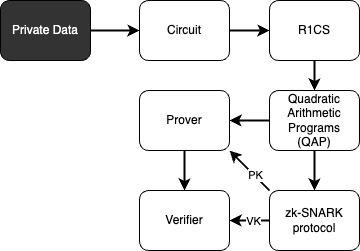
\includegraphics[width=0.4\textwidth]{figures/zk-snark-overview.jpg}
    \caption{Example Protocol Workflow for zk-SNARK}
    \label{fig:Fig 1}
\end{figure}

\subsection{Why zk-ML?}

A key advantage of certain ZKPs is their non-interactivity. The prover generates a proof the verifier will validate without any back-and-forth communication or involvement of additional parties. This avoids issues with latency or coordination interactive protocols like MPC face on public blockchains. ZKPs are also highly scalable with efficient verification, making them a natural fit for high-throughput blockchains.

In contrast, while FHE preserves privacy, the computational overhead of performing operations on FHE ciphertexts remains prohibitively expensive for most real-world AI use cases. MPC scales better than FHE but still requires rounds of interaction between nodes, presenting challenges on decentralized networks. Neither FHE or MPC provide the same level of correctness to verify every step of a computation.

ZKPs offer a lightweight and non-interactive approach to verify computations were done correctly on private inputs without exposing the exact computational steps or requiring participation by the verifier. This zero-knowledge property provides strong privacy guarantees for sensitive AI data and models.

The succinct nature and efficient verification of zk-SNARKs or zk-STARKs makes them seamlessly integrated into blockchain transactions. Nodes can easily verify proofs on-chain without needing to reproduce the underlying AI computations, often requiring orders of magnitude less computation to perform the verification.

For decentralized AI applications that require both privacy and verifiable correctness of results, zero-knowledge cryptography are an optimal cryptography primitive compared to alternatives. Their unique combination of succinct proofs, efficient verification, non-interactivity, and zero-knowledge privacy is compelling for blockchain-based AI.

In conclusion, while FHE and MPC offer robust cryptographic solutions, their applicability, efficiency, and synergistic potential with blockchain are not as useful as ZKP. Specifically, MPC might face significant challenges in scaling effectively in a distributed or decentralized context, given the bandwidth constraints of communications\endnote{Wang, W., Hoang, D.T., Hu, P., Xiong, Z., Niyato, D., Wang, P., Wen, Y., Kim, D.I. (2019). A Survey on Consensus Mechanisms and Mining Strategy Management in Blockchain Networks. IEEE Access, 7, 22328-22370. \url{https://ieeexplore.ieee.org/document/8629858} - Discusses limitations of MPC-based consensus protocols for blockchain including communication overhead.} \endnote{  Lu, S., Oikonomou, G., Zhang, H., Rahman, S., Koch, I. (2019). A Review of Distributed Consensus Protocols: Milestones and Challenges for Blockchain Networks. IEEE Internet of Things Journal, 6(2), 1674-1685. \url{https://ieeexplore.ieee.org/document/8374677} - Reviews limitations of MPC-based consensus for blockchain related to communication overhead.} and the physics constraints of transmission and coordination across the globe. These factors can severely limit the deployment of MPC in settings where rapid and extensive data exchange\endnote{Cachin, C., Vukolić, M. (2017). Blockchain Consensus Protocols in the Wild. arXiv preprint arXiv:1707.01873. \url{https://arxiv.org/abs/1707.01873} - Analyzes challenges of Byzantine consensus with MPC protocols on blockchain networks, including computation and communication costs.} is necessary. In contrast, zero-knowledge cryptography excel with their flexibility, privacy assurance, reduced trust assumptions, and swift verification processes, marking them as the most suitable cryptographic primitive for the complex convergence of AI and blockchain.\endnote{Zhang, R., Xue, R., Liu, L. (2019). Security and privacy on blockchain. ACM Computing Surveys (CSUR), 52(3), 1-34. \url{https://dl.acm.org/doi/10.1145/3316481} - Reviews blockchain privacy technologies and highlights superiority of ZKPs for blockchain systems.} As we progress toward a more pronounced intersection of these technologies, ZKP is poised to be instrumental in defining a decentralized, secure, and privacy-preserving foundation for AI-enhanced blockchain systems.

\section{zk-ML Workflow}
The integration of zero-knowledge machine learning (zk-ML)\endnote{Mohassel, P., \& Zhang, Y. (2017). SecureML: A System for Scalable Privacy-Preserving Machine Learning. 2017 IEEE Symposium on Security and Privacy (SP). doi:10.1109/sp.2017.12} into web3 is a sophisticated endeavor. One must have expertise in web3, machine learning, and zero knowledge cryptography which is narrow multidisciplinary intersection. The following is a non-exhaustive list of the steps a developer would need to take to bring a zk-ML application to fruition.
\subsection{AI Model Development}
The developer will need to start with a trained AI model. Today there are endless methods to create an AI model as referenced in our preliminary overly basic example.  Developers can pick frameworks in their favorite programming language or work with Python.\endnote{\url{https://docs.python.org/3/}}

Developers start from scratch by providing a large dataset which models the desired or expected behavior of the system. The dataset is generally a set of inputs to desired outputs. From here there are many strategies and methods to improve AI model performance. Reinforcement learning from human feedback for example is used as a part of today’s LLMs training process. The model accuracy, precision, recall, and other metrics are tracked as a model is trained to assess the fitness of the model for the end use case. 

Alternatively developers can build from an existing model in a process called fine tuning. This process usually involves reworking the desired output from a model by providing additional data or training techniques. This is an effective method as the data required for fine tuning is substantially less than starting from scratch. A large selection of “foundational models” are also available for fine tuning (such as Mistral 7B and GPT-2) which have been open sourced with a permissive license. This makes model creation significantly more accessible as creating a foundational model from scratch is cost prohibitive for most teams and use cases.

\subsection{Define the Computational Graph}
Since there are nearly endless toolsets, frameworks, and starting points to create and use AI models, an AI model universal exchange format is generally used rather than native support of popular ML frameworks by the tools in the next step (Circuit Generation). The Open Neural Network Exchange (ONNX)\endnote{\url{https://onnx.ai/}} was created to promote innovation and collaboration in the AI sector\endnote{\url{https://en.wikipedia.org/wiki/Open_Neural_Network_Exchange}} and is the most widely used exchange format today. It is a concise representation of the structure, weights, and biases of the AI model.

PyTorch, Tensorflow and other frameworks provide functionality to export a trained AI model to ONNX. It should be noted this is not a perfect 1:1 process and verification should be performed on the ONNX export to confirm it meets performance requirements of the end use case.
\subsection{Circuit Generation}
With a universal representation of the AI model in hand, the next step is to derive a circuit and set of constraints from the model. Firstly a computational graph of the model is created.  A computational graph is a representation of the operations (such as addition, multiplication, etc.) as nodes and data as edges. In the context of an AI model, this graph represents the flow of computations through the layers and functions of the model. 

Optimizations can be made once in this representation. Sparseness can be removed where possible and approximations of nonlinearities are made into lookup tables. Floating point arithmetic is scaled at the expense of accuracy.  From here a nearly 1:1 representation of the model is outlaid in a circuit.
\begin{figure}[!ht]
    \centering
    \scalebox{0.65}{

\tikz{
\tikzstyle{block}=[draw, inner sep=0pt, outer sep=0pt, minimum width=3.3cm, minimum height=.85cm, rounded corners=1mm, align=center]

\node[block] (a) {Input Layer};
\node[block, below=3mm of a] (b) {Quantization};
\node[block, below=3mm of b] (c) {Encoding};
\node[block, below=3mm of c] (d) {Arithmetic Circuit};
\node[block, below=3mm of d] (e) {Decoding};
\node[block, below=3mm of e] (f) {Output Layer};
\node[block, below=3mm of f] (g) {Proving Stage};
\node[block, below=3mm of g] (h) {Verification Stage};

%--------------------------
\node[block, left=2cm of h, minimum width=2.5cm, fill=black!60, text=white] (ver) {Verifier};
\node[block, below=2cm of ver, fill=black!60, text=white, rounded corners=4.3mm] (pu) {Proof Unverified};
\node[block, left=2cm of a, minimum width=2.5cm, fill=black!60, text=white, rounded corners=4.3mm] (pr) {Prover};

\node[block, minimum size=1.85cm, rotate=45, rounded corners=0pt] (vp) at (pu-|h) {};
\node at (vp) {Valid Proof?};

\node[block, right=2cm of h, minimum width=2.5cm, fill=none, draw=none, text=white] (verf) {};
\node[block, below=2cm of verf,  fill=black!60, text=white, rounded corners=4.3mm] (pv) {Proof Verified};

%-------------------
\draw[-triangle 45] ($(a.west)+(-1,0)$)--node[pos=0, left] {\small Input} (a.west);
\draw[-triangle 45] (a.east)--++(1,0) |- node[pos=0.25, right, align=left, font=\small] {Data to be processed} (b.east);
\draw[-triangle 45] (b.west)--++(-1,0) |- node[pos=0.25, left, align=right, font=\small] {Convert to fixed point\\numerical representation} (c.west);
\draw[-triangle 45] (c.east)--++(1,0) |- node[pos=0.25, right, align=left, font=\small] {Encode} (d.east);
\draw[-triangle 45] (d.west)--++(-1,0) |- node[pos=0.25, left, align=right, font=\small] {Process encoded\\ input data} (e.west);
\draw[-triangle 45] (e.east)--++(1,0) |- node[pos=0.25, right, align=left, font=\small] {Decode Arithmetic\\ Circuit Output Data} (f.east);
\draw[-triangle 45] (f.west)--++(-1,0) |- node[pos=0.25, left, align=right, font=\small] {Submit to \\Proving Stage} (g.west);
\draw[-triangle 45] (g.east)--++(1,0) |- node[pos=0.25, right, align=left, font=\small] {} (h.east);
\draw[-triangle 45] (h)--(ver);
\draw[-triangle 45] (ver.south)--++(0,-.5) -| (vp.north east);
\draw[-triangle 45] (vp.north west)--node[fill=white] {\textbf{No}} (pu);
\draw[-triangle 45] (vp.south east)--node[fill=white] {\textbf{Yes}} (pv);
}
}

    \caption{Proof Generation to Verification data flow within zkml}
    \label{fig:Fig 3}
\end{figure}

Currently ezkl is the most feature complete and widely used framework for this process. Its implementation uses halo2 to generate proving and verification keys. Halo2 is a zero-knowledge proof protocol that enables the construction of proofs without a trusted setup.  It aims to facilitate the recursive composition of zk-SNARKs, allowing for more scalable and efficient proofs. Halo2 represents the next generation of zk-SNARK technology after the original Halo protocol.\endnote{\url{https://github.com/zcash/halo2/tree/main}} 

Depending on the proving backend used, a trusted setup may be required during the circuit creation process. Halo2 eliminates this requirement by using recursive composition of proofs, which can create a system where proofs can be verified without a trusted setup. See the Security section for this in more detail.
\subsection{Off-chain Compute and Proof Generation}
With a proving key in hand, a proof is generated making an explicit claim $[y]$ output was obtained from $[z]$ model from $[x]$ input. The proof generation process is computationally intensive as operations in addition to the inference output must be calculated to show the computation has been performed correctly.
\subsection{On-chain Verification}
With a proof in hand and the aforementioned verifier key, a computationally cheap operation is performed to verify the claim $[x]$ input run through $[z]$ model obtained $[y]$ output. This typically occurs in a verifier smart contract where the verifying key has been committed on chain and cannot be changed. Since the verifying key is locked and represents a single AI model, the contract will only verify output from this exact AI model and only output which has been computed correctly.
\subsection{On-chain Execution}
Since the output has now been verified it can be used in on-chain applications. No AI output exists in a vacuum, it has meaning in a context. An on-chain application will interpret the output and perform an action. This can take many forms such as a trade, a swap, minting of an NFT, release of funds, liquidation event, pausing of a protocol, and loan issuance just to name a few.
\subsection{Scalability and Cost Efficiency}
Utilizing AI inferences and executing smart contracts on Layer 1 blockchains can become exceedingly expensive, particularly when the volume of data storage grows. For instance, if ChatGPT were to operate on Ethereum's Layer 1, the gas fees alone could surpass \$60 million USD daily,\endnote{By August 2023, daily queries to ChatGPT increased to over 60 million, leading to increase in costs. \url{https://nerdynav.com/chatgpt-statistics/}} not accounting for the additional costs of computational GPU infrastructure.

\subsection{Cross-chain Execution}
Since blockchains are often siloed, creating an application which functions seamlessly across multiple chains requires interaction with different blockchain protocols and smart contract systems. Currently no frameworks, protocols, or standards exist for AI model use in applications across blockchains.

\textit{Interoperability:} Developing a cross-chain communication protocol that enables blockchains with different consensus mechanisms and data structures to interact with AI models.

\textit{Smart Contract Compatibility:} Writing smart contracts which execute and understand the AI model’s outputs in various smart contract programming languages (e.g., Solidity for Ethereum, Rust for Solana).

\textit{Data Formats:} Standards must be established to ensure AI will produce outputs that are actionable within the context of different blockchain protocols and applications. Human centered models with output such as text are not actionable by blockchains.

\textit{Security Concerns:} The system must ensure that the AI’s predictions or outputs are as intended, the AI model and its outputs must be secure against manipulation and errors

\textit{Scalability Challenges:} AI must operate within the transaction capacity of blockchains to avoid network congestion and maintain manageable transaction fees. As AI usecases continue to grow, their onchain transactions will follow.

\textit{Price Variability:} Keeping transaction fees (gas costs) manageable, especially during periods of network congestion.  Costs of deploying proving circuits, contracts, and keys across multiple chains may prove to be cost prohibitive.

Building an AI model with on-chain execution across multiple blockchains is an intricate task that requires sophisticated technical solutions to overcome interoperability, standardization, security, and scalability challenges. The actual deployment demands of independent operators would be a considerable investment in both technical development and cross-chain operational costs of both the platform and it’s users.

\subsection{Alternative Workflows}
The examined workflow is not universal and other novel approaches have been used. The following is a non exhaustive list of approaches seen in use today.

One approach transpiles ONNX files to Cairo\endnote{\url{https://docs.starknet.io/documentation/architecture_and_concepts/Smart_Contracts/cairo-and-sierra/}} (a turing complete programming language for writing provable programs) and uses the Starknet zkVM\endnote{\url{https://docs.starknet.io/documentation/}} to verify the computation. Models are publicly deployed and can be used by anyone following the protocol. This approach may expose parts of the AI model publicly and increase the chances the AI models will be reverse engineered.

Another approach creates economic incentives within a network for nodes to create and distribute machine intelligence. Miners within the network create value by completing requests for inference with a locally hosted AI model and return the output to the client. Rather than cryptographic verification of the output, the network relies on a series of Validators to ensure the integrity and quality of data and models within the network. The project also has a focus on the continual improvement of models through crowdsourcing of data which is in direct opposition of verifying an exact model was used for an inference.

An additional approach is a consensus based voting scheme where nodes complete work and validator or “interrogator” nodes review inference output on a random or complaint driven basis. This method only works with open source models as the validator node needs a source of truth, the model itself, to rerun and confirm the output. In cases where the model is private, the validator nodes do not have access and cannot perform this check without the model node’s disclosure of additional model details. This defeats the purpose of model privacy and is not a viable architecture to support private model inference execution. The same line of reasoning applies to optimistic methods of dispute resolution, not to mention the delay of inference settlement during a claim window.

\subsection{Summary}
The current process for integrating zero-knowledge machine learning (zk-ML) into applications is complex and resource-intensive, both computationally and in engineering effort. From the outset, AI model development requires a significant amount of data and computational power, particularly when building models from scratch. This foundational stage involves training models to emulate desired behaviors, optimizing performance through various strategies like reinforcement learning, and fine-tuning pre-existing models, which, while less data-intensive, still requires considerable computational resources. Moreover, the translation of these models into a universally acceptable format, such as ONNX, is not straightforward and necessitates thorough verification to ensure performance standards are met for the intended use case.

The complexity escalates with the transition to circuit generation, where the AI model must be represented as a computational graph to derive a circuit and constraints, a process which demands extensive optimizations and approximations. Implementing this within a zk-SNARK framework such as ezkl with halo2, although efficient in eliminating the need for a trusted setup, still involves the generation of proving and verification keys. The creation of proofs are computationally demanding, ranging from a 100x-1000x overhead in addition to the initial computation being proven. On-chain execution further complicates matters, requiring secure, interpretable, and scalable smart contract integrations across multiple blockchains, each with their own protocols. The associated costs and technical challenges of ensuring data integrity, security, and execution verification only add to the overall burden, demanding significant investment in development and infrastructure to enable seamless AI functionality across diverse blockchain ecosystems.

\begin{figure}[!ht]
    \centering
    \scalebox{0.65}{
\tikz{
\tikzstyle{block}=[draw, inner sep=0pt, outer sep=0pt, minimum width=2.2cm, minimum height=1.2cm, rounded corners=1mm, align=center]

\node[block] (a) {On-chain\\Verification};
\node[block,right=.5cm of a] (b) {Proof\\Storage}; 
\node[block, right=.5cm of b] (c) {Execution\\Action}; 
%---------
\node[draw, densely dotted, thick, minimum width=8.5cm, minimum height=2.3cm, rounded corners=2mm] (l1) at (b)  {};


\node[above, anchor=south west] at ([xshift=0mm]l1.north west) {\scriptsize\textbf{L1 / repeated for each chain}};

\node[block, minimum width=2.5cm, left=3cm of a] (ai) {Al Operator /\\Application};

\begin{scope}[xshift=-2.5cm,yshift=3.3cm]
\foreach \i in {1,1.7,...,10}{
\foreach \j in {0,-.5}{
\node[fill=black, inner sep=2.3pt] at (\i,\j) {};
}
}   
\end{scope}

\node[align=left, anchor=west, font=\small] at ([yshift=2.45cm]ai.north west) {\textbf{End users}\\\textbf{Al prediction consumers}};
%-------------
\draw[-triangle 45] (ai)--node[fill=white, font=\footnotesize, align=center, pos=.45] {Circuitization\\of AI Model} (a);

\draw[triangle 45-] ([yshift=-4mm]l1.80)--+(0,1.5);
}    
}

    \caption{Current state of on-chain zk-ML}
    \label{fig:Fig 4}
\end{figure}

\section{Omron}
Omron Network offers a transformative approach for AI operators seeking to transition their off-chain AI models onto blockchain networks while safeguarding their proprietary algorithms. This framework streamlines the intricate process of model conversion, enabling rapid deployment across multiple blockchain ecosystems. It serves as a seamless bridge between the off-chain world of AI and the on-chain realm, ensuring intellectual property remains veiled through the use of zero-knowledge cryptography. By providing a secure and efficient payment infrastructure, Omron facilitates atomic value exchange for AI services, paving the way for a new era of autonomous AI agents interacting within the blockchain space.

For consumers of AI predictions, Omron offers an additional layer of assurance by eliminating trust assumptions. They confidently rely on the network to validate inputs are processed using the correct and intended AI model, with a cryptographic guarantee of faithful execution.  As a result, consumers of AI services benefit from a transparent, trust-minimized environment where AI predictions are verified, reducing the need for blind trust in the operators' execution.
\subsection{Technical Architecture}
To address current blockchain limitations and challenges of running on-chain Neural Networks, Omron is designed to serve as a conduit between off-chain and on-chain architectures. Taking a forward-looking approach, the Omron architecture is inherently modular, a design philosophy which allows each component of the system to be individually updated or replaced.

\begin{figure}[!ht]
    \centering
    \include{figures/Omron-overview}
    \caption{Omron Overview}
    \label{fig:Fig 5}
\end{figure}
This adaptability is a core characteristic, anticipating the need to integrate advanced AI models and alternative solutions as they emerge in the dynamic AI and blockchain landscape.
\subsection{Off-Chain Architecture}
\textit{Node Pools: }The off-chain infrastructure and computational power of Omron is based around node pools. These pools consist of registered nodes that are assigned to process specific models' inference workloads. After registration, a model node becomes part of the available workforce. A node may service multiple models, and it is incumbent upon the node operator to ensure the successful completion of assigned tasks. Nodes pledge a certain amount of computational power and time to the network. With the computational requirements of workloads being predetermined, the network allocates tasks accordingly and does not exceed a node's capacity. A node is expected to fulfill its commitments within the epoch it is registered. Any failure to perform, or indication of unavailability, may result in penalties to the node.

\begin{figure}[!ht]
    \centering
    \scalebox{0.50}{
\tikz{
\tikzstyle{block}=[draw, inner sep=0pt, outer sep=0pt, minimum width=1.8cm, minimum height=1.2cm, rounded corners=1mm, align=center, fill=black!50]

\node[draw, densely dotted, thick, minimum width=8cm, minimum height=1.7cm, rounded corners=2mm] (r1) at (0,0)  {};
\node[draw, densely dotted, thick, minimum width=8cm, minimum height=1.7cm, rounded corners=2mm, left=3mm of r1] (r2) {};

\node[fill=white, anchor=west, xshift=2mm] at (r2.north west) {\footnotesize\textbf{Node Pool}};

\node[block, anchor=west, text=white] (a) at ([xshift=3mm]r1.west) {Node A};
\node[block,right=.3cm of a, text=white] (b) {Node B}; 

\node[block, anchor=west, text=white] (a1) at ([xshift=3mm]r2.west) {Node A};
\node[block,below=.55cm of a1, text=white] (b1) {Node B}; 
% %---------
\node[minimum width=1.75cm, minimum height=1.2cm, anchor=south west] (1) at ([yshift=3mm]r2.north west) {};
\draw (1.north west)--coordinate[pos=1] (w) ($(1.west)+(.5,0)$)--(1.south west)--(1.south east)--coordinate[pos=1] (z) ($(1.east)+(.5,0)$)--(1.north east)--cycle;
\node[align=center, font=\scriptsize] at($(w)!.4!(z)$) {Workload\\1};

\node[minimum width=1.75cm, minimum height=1.2cm, right=1.3mm of 1] (1) {};
\draw (1.north west)--coordinate[pos=1] (w) ($(1.west)+(.5,0)$)--(1.south west)--(1.south east)--coordinate[pos=1] (z) ($(1.east)+(.5,0)$)--(1.north east)--cycle;

\node[minimum width=1.75cm, minimum height=1.2cm, right=1.3mm of 1] (1) {};
\draw (1.north west)--coordinate[pos=1] (w) ($(1.west)+(.5,0)$)--(1.south west)--(1.south east)--coordinate[pos=1] (z) ($(1.east)+(.5,0)$)--(1.north east)--cycle;
\node[align=center, font=\scriptsize] at($(w)!.4!(z)$) {Workload\\2};

\node[minimum width=1.75cm, minimum height=1.2cm, right=1.3mm of 1] (1) {};
\draw (1.north west)--coordinate[pos=1] (w) ($(1.west)+(.5,0)$)--(1.south west)--(1.south east)--coordinate[pos=1] (z) ($(1.east)+(.5,0)$)--(1.north east)--cycle;
\node[align=center, font=\scriptsize] at($(w)!.4!(z)$) {Workload\\3\\Workload\\4};



\node[minimum width=1.75cm, minimum height=1.2cm, anchor=south west] (1) at ([yshift=3mm]r1.north west) {};
\draw (1.north west)--coordinate[pos=1] (w) ($(1.west)+(.5,0)$)--(1.south west)--(1.south east)--coordinate[pos=1] (z) ($(1.east)+(.5,0)$)--(1.north east)--cycle;
\node[align=center, font=\scriptsize] at($(w)!.4!(z)$) {Workload\\5};

\node[minimum width=1.75cm, minimum height=1.2cm, right=1.3mm of 1] (1) {};
\draw (1.north west)--coordinate[pos=1] (w) ($(1.west)+(.5,0)$)--(1.south west)--(1.south east)--coordinate[pos=1] (z) ($(1.east)+(.5,0)$)--(1.north east)--cycle;
\node[align=center, font=\scriptsize] at($(w)!.4!(z)$) {Workload\\6};

\node[minimum width=1.75cm, minimum height=1.2cm, right=1.3mm of 1] (1) {};
\draw (1.north west)--coordinate[pos=1] (w) ($(1.west)+(.5,0)$)--(1.south west)--(1.south east)--coordinate[pos=1] (z) ($(1.east)+(.5,0)$)--(1.north east)--cycle;
\node[align=center, font=\scriptsize] at($(w)!.4!(z)$) {Workload\\7\\Workload\\8};

\node[minimum width=1.75cm, minimum height=1.2cm, right=1.3mm of 1] (1) {};
\draw (1.north west)--coordinate[pos=1] (w) ($(1.west)+(.5,0)$)--(1.south west)--(1.south east)--coordinate[pos=1] (z) ($(1.east)+(.5,0)$)--(1.north east)--cycle;
\node[align=center, font=\scriptsize] at($(w)!.4!(z)$) {Workload\\9\\Workload\\10};

%---------------
\node[above=1.6cm] at (r2.north) {Epoch 1};
\node[above=1.6cm] at (r1.north) {Epoch 2};
% Paths
\draw[-triangle 45] (b1)-| node[pos=.25, fill=white] {\small \textbf{Node Registers based on workload}} (b);
}
}

    \caption{Epoch transition with new Node registration}
    \label{fig:Fig 6}
\end{figure}

\subsection{Persistent Storage}
Due to the considerable size of input and outputs from AI models, external persistent storage is required. Depending on the ultimate end use case of the output, storage within Omron may not be required. An example is an NFT image generated with a diffusion model. The hash of the image can be verified and stored onchain with the image being stored on Arweave or other decentralized storage networks.

\subsection{Aggregation Circuits}
As the complexity of a model increases, so does the size of its associated zk-circuit, resulting in larger proofs. To manage this, aggregation circuits are utilized to amalgamate multiple proofs into a singular, more concise proof that can be submitted on-chain, along with the corresponding output data. This technique also permits the batching of related inferences, enhancing efficiency and reducing the on-chain data storage footprint.

\subsection{On-chain Architecture}
The on-chain component of the Omron system acts as the interface for end users and decentralized applications (dApps).  Users or dApps submit workloads, which include all necessary details like input, precommitment, and destination. This on-chain architecture consists of three main components: The Inference Market, Model Registry, and Verifier Contracts.

\subsection{Inference Market}
The ecosystem is anchored by an Inference Market. The protocol has a native queue of AI/ML workloads. A workload can be thought of as an end to end AI/ML Inference. Each workload specifies all required details to complete it, such as input data, specific AI model for execution, output data requirements or on-chain execution. Workloads posted to the network are priced according to their computational complexity.

\subsection{Model Registry}
After circuitizing a model with the Omron SDK, its creator will register it on the network. This defines the required input and output data format, computational cost of inferences on the model (proportional to cost of compute for an inference) and the verification key for use in a verification contract upon completion of each inference from the model.

\subsection{Model Node Pool Registration}
In order to complete inference workloads for a model, a model node must register its intent to complete workloads for specific models. Once registered the node is added to the pool of available nodes. Nodes may be registered to service multiple models, but it is the responsibility of the operator to ensure the node completes assigned workloads.

\begin{figure}[!ht]
    \centering
    \scalebox{0.65}{
\tikz{
\tikzstyle{block}=[draw, inner sep=0pt, outer sep=0pt, minimum width=2.2cm, minimum height=1.2cm, rounded corners=1mm, align=center]

\node[block, fill=black!50, text=white] (a) {Model A};
\node[block, fill=black!50, text=white, right=.5cm of a] (b) {Model B};
\node[block, fill=black!50, text=white, below=.5cm of a] (c) {Model C};

\node[block,  left=2cm of a] (na) {Node A};
\node[block,  below=.5cm of na] (nb) {Node B};

%---------
\coordinate (p) at ($(a.west)!.5!(c.west)$);
\node[draw, dashed, anchor=west, minimum width=5.8cm, minimum height=3.5cm, rounded corners=2mm, label={above:Node Pool}] at ($(p)+(-.5,0)$)  {};
%-------------
\draw[-triangle 45] (na)--(a);
\draw[-triangle 45] (nb)--(c);
\draw[-triangle 45] (nb.east)--++(.7,0) |- (a.195);
}
}

    \caption{Model Registration}
    \label{fig:Fig 7}
\end{figure}
The network implement sets of blocks, called epochs, in which a registered node must be available. Nodes which register in the current epoch are activated during the following epoch. Model nodes commit compute units per unit of time to the network. Since the compute units for a workload is known ahead of time (see “Transactional Cost” section) the network delegates workloads to fill but not exceed its compute capacity. 

It is the expectation a model node will complete delegated workloads during a registered epoch. Model nodes which fail to complete work while registered or otherwise shown to be unavailable will face a penalty.

\subsection{Model Vetting}

As Omron will be an open permission-less network, no party (or even Inference Labs) can decide which models should or shouldn’t be available on the network. Instead an economic system determines how “good” a model is. This is crucial to retain an open and fair censorship free network.

Verified backtesting is published by the model creator and made available to the public. Users get a guarantee the model will perform a certain way under set circumstances rather than relying on blind trust in published accuracy, precision and recall values. While the provided examples may not be representative of real world use cases as it is self published by the creator, this is clearly a move in the right direction. Users also submit inferences one at a time, with no upfront commitments or complicated setup to quickly verify the usefulness of the model for their application.

Aggregating onchain historical usage of a model results in a proof of its usefulness. How “good” a model is can be answered by its frequency of use, inference by a diverse set of applications and users, and repeat use of a model by a user. In the same way an open source software package can be evaluated by the number of other projects which depend on it (and subsequently how “good” those packages are).

The network implements a non-zero registration fee for models to prevent flooding of the network with unusable or non-existent models.

\section{Network Operation}
\begin{figure}[!ht]
    \centering
    \scalebox{0.65}{
\tikz{
\node[scale=2.5, label={[label distance=0mm]below:Consumer}, inner sep=0pt] (cus) {\faUser};

\draw[dashed] (0,-1.3)--
coordinate[pos=.1] (a1)
coordinate[pos=.25] (a2)
coordinate[pos=.9] (a3)
+(0,-6);

\draw[dashed] (4.5,-1.3)--node[pos=0, above=3mm, align=center] {Omnichain\\L1, L2, L3}
coordinate[pos=.1] (b1)
coordinate[pos=.25] (b2)
coordinate[pos=.9] (b3)
coordinate[pos=.75] (b4)
+(0,-6);

\draw[dashed] (9,-1.3)--node[pos=0, above=3mm, align=center] {zk-VIN}
coordinate[pos=.1] (c1)
coordinate[pos=.25] (c2)
coordinate[pos=.9] (c3)
coordinate[pos=.4] (c5)
coordinate[pos=.55] (c6)
+(0,-6);

\draw[dashed] (13.5,-1.3)--node[pos=0, above=3mm, align=center] {Node\\(dApp)}
coordinate[pos=.1] (d1)
coordinate[pos=.25] (d2)
coordinate[pos=.9] (d3)
coordinate[pos=.75] (d4)
coordinate[pos=.4] (d5)
coordinate[pos=.55] (d6)
+(0,-6);


\draw[-triangle 45] (a1)--node[fill=white, font=\footnotesize] {[Input, precommitment]} (b1);
\draw[-triangle 45] (a2)--node[fill=white, font=\small] {[Input, computation payment, output destination]} (c2);
\draw[triangle 45-] (a3)--node[fill=white, font=\footnotesize] {On-chain state updated} (b3);
\draw[triangle 45-triangle 45] (b4)--node[pos=.255,fill=white, font=\footnotesize, align=center] {Verify proof\\Rollup Verified Output} node[pos=.75,fill=white, font=\footnotesize, align=center] {Remit payment} (d4);
\draw[-triangle 45] (c5)--node[fill=white, font=\footnotesize, align=center] {Delegate worker} (d5);
\draw[triangle 45-] (c6)--node[fill=white, font=\footnotesize, align=center] {Perform inference\\Calculate Proof} (d6);
}    
}

    \caption{Overview of interaction between Consumers, Networks, Omron, and Decentralized Application}
    \label{fig:Fig 8}
\end{figure}
\subsection{State and Data Commitment}
To start an inference, a commitment is made on chain by submitting the input data the inference shall be run on. This may include data from both on chain and off chain sources. This data is then attested as the input to the model when the proof and output is submitted to Omron. The commitment also defines which model the data should be run on.

\subsection{Workload Delegation}
The network delegates a model node to complete the workload. A model node is selected from the node pool using a deterministic process. This provides a guarantee the inference will be completed or nodes which are unable or unavailable to complete a workload are removed from the pool.

If no model node is available to complete the workload it will remain undelegated until it either expires after a set amount of time or a node is registered to complete the workload.

\subsection{Inference and Proof Generation}
Once inference details have been posted and committed to the network, it is assigned to an available node. The node then performs the inference and generates a zero knowledge proof using a pre-generated zk-circuit for the exact model snapshot. The proof is an explicit claim the output was achieved by running the precommitted data through the particular model. Proofs are then submitted to Omron along with the output to be verified on-chain.

\subsection{Verification Contract}

To ensure the integrity of on-chain AI model inferences, Verification Contracts are employed. Each AI model verified on-chain is paired with a unique verification key, which is stored within these contracts. The Omron SDK is responsible for the generation and deployment of model-specific contracts alongside their corresponding circuitized AI models. The contract accepts two main inputs - a byte array containing proof data, and an array of public input/output instances. It then executes assembly code to process the proof and input data, performing cryptographic operations to verify the proof.  If the proof is valid, the contract returns 1. If invalid the transaction is reverted.

\subsection{Verification and Payment Layer}
Proofs submitted to Omron are stored and verified on the app chain. Payments which were remitted and locked beforehand for the compensation of compute are then transferred to the worker which has completed the inference. Payment fees are calculated with a base rate proportional to the memory usage and compute time required to complete the off chain operations. Fees are dynamically adjusted based on overall transaction volume on the network and then further based on the demand for each model and the number of available nodes which can perform inference on said model.

Royalties will be remitted to model creators based on a preset fee for model usage (either percentage or flat rate based) each time a model is used for inference within Omron. Protocol fees will be remitted on each transaction to support the overall development and ecosystem of Omron.

\subsection{Execution Layer}
Output from inferences are executed in one of the following places. Directly on Omron via deployed smart contracts. This option has the lowest fees and fastest execution time. The second option is to rollup the inference output, have a dapp smart contract on any other chain interpret the output and perform an on chain action based on the results. This could be anything from a swap to a DAO administrative action.

The decision between the two options is up to the application developer and will be determined based on the specifics of the end use case.

There is a third option which requires no execution. Some inference output may be used off chain or not require any execution, in which case the output will remain and no further action is required by the network.

\subsection{Data Availability}
Input data, output data and proofs of AI execution are large and expensive to store on L1. Below is a comparison of the cost of data storage. A reference of a 1kB proof size is used. This assumes storing one uint256 takes 20k of gas, with 1kb therefore requiring 640,000 gas.

\vspace{4mm}
\begin{tabular}{|p{47pt}|p{90pt}|p{66pt}|}
\hline \textbf{Network} & \textbf{Fee in Native Token} & \textbf{Cost in \$USD (October 2023)} \\
\hline Ethereum & 0.032ETH (gas@0.50gwei) & $\$ 54.40$ USD \\
\hline Polygon & 0.08MATIC (gas@125gwei) & $\$ 0.048$ USD \\
\hline BNB Smart Chain & 0.0032BNB (gas@0.5gwei) & $\$ 0.71$ USD \\
\hline Arweave & 0.00021 AR & $\$ 0.001$ USD \\
\hline Omron (estimated) & 0.0032VIN (gas@0.5gwei) & $<\$0.01$ USD (targeted) \\
\hline
\end{tabular}

\vspace{4mm}
Gas fees across networks are inconsistent and unpredictable. In contrast to an L2, it can cost 100-1000x on ethereum L1 to verify and store a proof and this can vary depending on network traffic. While fluctuations in the cost cannot be eliminated, they can be minimized by using Omron as a data availability layer for proof storage.

In cases of private models the raw computations (end to end method to achieve output from an input) may not be repeatable in full by any node on the network as not all data will be available to each node. Inputs for inferences may be hashed or obscured publicly and proprietary models will remain private. The verification keys and proofs must exist on chain to confirm the validity of the output from the models.

\subsection{Transactional Cost}
Computational cost will be calculated in Gb-Sec which is the amount of CPU, RAM and time used to compute the inference and the zk proof to verify the computation. Since inference is generally a bound computational operation (along with the proof generation) most inferences will be a fixed cost in Gb-Sec.

\subsection{Ease of Management and Deployment}
As the complexity of dapps and protocols increase, the complexity and cost of managing and maintaining these applications also increases. Web3 teams are already faced with challenges in managing multi-chain applications, adding zero knowledge and machine learning only increases complexity further. A solution which reduces the complexity and domain knowledge required to deliver and operate an application will be crucial to the long term success of the space.

\subsection{Upgradability}
Technical sovereignty is a fundamental requirement as the state of AI is rapidly developing. Omron will require frequent upgrades and migrations to include new features and improvements. There must be a clear path for users to migrate their assets between versions in a trustless fashion and easily migrate any dapps to the latest version.

\subsection{Reputation System}
The Omron network is set to incorporate a comprehensive Reputation System, designed to enhance transparency and accountability among AI Model providers and computational nodes while providing the benefits of being censorship resistant. This system is structured to capture and disseminate feedback from consumers, granting them the ability to make informed decisions based on the aggregated performance data of AI Model operators. The core of this system will be the Validator Reports, which are expected to be a critical element in establishing and maintaining the credibility of AI Model reputations.

Within this framework, the Reputation System will track and publicize a variety of metrics, available both on-chain for smart contract interactions and off-chain for in-depth analysis. Key performance indicators for AI Model operators will include:

Let $R$ be the reputation score for an AI Model operator. This score can be a weighted sum of several factors:

Volume of Inference Requests ($V$):

$V_{\text{assigned}}$ : Total number of assigned inference requests to a specific Al Model.

$V_{\text {completed }}$ Total number of completed requests by an AI Model, offering insights into reliability  when contrasted with the total assignments.

Fulfilment Rate $(F)$:

$F=\displaystyle \frac{V_{\text {complicated}}}{V_{\text {assigned}}}:$ A tally of the requests successfully completed by an Al Model, offering insights into reliability

Fulfilment rate ($F$)
Validation Score $\left(S^{\prime}\right)$ :
$S_{\text {accepted }}$ : Total number of accepted requests for validation by the consensus mechanism.
$S=\displaystyle \frac{S_{\text {accepted }}}{V_{\text {completed }}}$ : A ratio of the requests validated by Omron consensus mechanisms, providing a measure of the Al Model's authenticity and accuracy.

Response Time $\left(I^{\prime}\right)$ :
$$
T=\frac{\sum \text { (response times) }}{V_{\text {completed }}} \text { : }
$$
An average calculation of the time taken by an Al Model to respond, reflecting on the operator's efficiency.

Backtesting samples $(B)$ :
$B_{\text {points:}}$ Total data points per backtest
$B_{\text {tests: }}$ Total number of backtests
$$
B=B_{\text {points }} \times B_{\text {tests}}
$$

Penalty Incidence $(P)$ :
$P_{\text {incurred }}$ : Total penalties incurred by the Al Model operator. 

$P=\displaystyle \frac{P_{\text {incurred}}}{V_{\text {assigned}}}$ The ratio of penalties to assigned requests, indicating reliability.

The overall reputation score   could then be computed by applying weights to these factors, reflecting their relative importance:

$$
\begin{aligned}
& R=w_1 \cdot F+w_2 \cdot S+w_3 \cdot\left(1-T_{\text {normalized }}\right) \\ & +w_4 \cdot B+w_5 \cdot\left(1-P_{\text {normalized }}\right)
\end{aligned}
$$

Here, $w_1, w_2, w_3, w_4$ and $w_5$ are the weights assigned to each factor, and $T_{\text {normalized }}$ and $P_{\text {normalized }}$ are the normalized response time and penalty ratios.

These metrics are aimed at fostering a positive feedback loop where high-reputation services are naturally driven to maintain exceptional standards of service. Negative feedback and financial penalties pose substantial risks to an operator's market standing, thereby creating strong incentives for consistent, high-quality performance. The Omron Reputation System is envisioned as a pivotal component in promoting a self-reinforcing cycle of identifying AI models with high standings while motivating them to uphold credibility and superior performance within the ecosystem.

\subsection{Cross Chain Communication}
Cross-chain communication is a fundamental aspect of the Omron architecture, allowing disparate blockchain networks to interact and share information. This interoperability is crucial for creating a more connected and functional decentralized inference ecosystem.

Many base chain and scalability platforms offer chain development kits (CDKs) that are designed to be highly modular and adaptable, enabling the construction and integration of diverse blockchain ecosystems.  Omron will roll out a application-specific chain to meet the needs of AI Operators such as support for larger contracts (could run up to MB in size), data availability, and tokenomics all while leveraging shared validators and inheriting chain security. Additionally, the EVM can be upgraded to support additional cryptographic primitives to ensure compatibility with future zk proving systems. 

For AI models, cross-chain communication methods provide a seamless way to distribute verified outputs across different networks, ensuring that the value generated on one chain can be recognized and utilized on another. With the growth of decentralized finance (DeFi), non-fungible tokens (NFTs), and other blockchain-based innovations, operating across chains is becoming the standard requirement for new projects in the space. The low cost and secure nature of these cross-chain communications protocols ensure they are accessible to a wide range of projects, from small startups to large enterprises, furthering the vision of an interoperable and open Web3 ecosystem.

\begin{figure}[!ht]
    \centering
    \scalebox{0.5}{
\tikz{
\tikzstyle{block}=[draw, inner sep=0pt, outer sep=0pt, minimum width=2.2cm, minimum height=1.2cm, rounded corners=2mm, align=center]

\begin{scope}[on above layer]
\node[block,  rounded corners=6mm] (a) {dApp\\Contracts};  
\end{scope}

%---------
\node[draw,fill=white, densely dotted,  thick, minimum width=5.5cm, minimum height=2.5cm, rounded corners=2mm] (ls1) at (a)  {};
\begin{scope}[on behind layer]
\node[draw, densely dotted, thick,fill=white, minimum width=5.5cm, minimum height=2.5cm, rounded corners=2mm] (ls2) at ($(a)+(-.35,.35)$)  {};
\end{scope}
\begin{scope}[on background layer]
\node[draw, densely dotted,thick, fill=white, minimum width=5.5cm, minimum height=2.5cm, rounded corners=2mm] (ls3) at ($(a)+(-.7,.7)$)  {};
\end{scope}

\node[fill=white, anchor=west] at ([xshift=3mm]ls1.north west) {\scriptsize{L1s ie. Ethereum, Near, Solana}};
\node[fill=white, anchor=west] at ([xshift=3mm]ls2.north west) {\scriptsize{L2s ie. Polygon, Arb, Stark}};
\node[fill=white, anchor=west] at ([xshift=3mm]ls3.north west) {\scriptsize{L3s ie. Appchains}};

\node[block, minimum width=3.5cm, minimum height=2cm, left=4.5cm of a] (rs)  {Rollup\\\footnotesize(sequencer, verifier, msg)};

\node[block, minimum width=3.5cm, minimum height=2cm, above=2.5cm of rs] (mr)  {Model registry\\Inference market};
\node[block, minimum width=3.5cm, minimum height=2cm, right=.6cm of mr] (np)  {Node pool\\Worker};
\node[block, minimum width=3.5cm, minimum height=2cm, right=.6cm of np] (ua)  {Unique AI Model\\Verification Contract};

\node[dashed, draw, minimum width=12.5cm, minimum height=2.5cm, rounded corners=2mm] (rec) at (np) {};
\node[anchor=west, above, xshift=7mm] at (rec.north west) {\textbf{zk-VIN}};

\node[left=2cm of rs, scale=3.5] (cus) {\faUser};

\begin{scope}[on above layer]
\node[block, fill=white, rounded corners=6mm,  above=2.7cm of cus] (om) {Omnichain\\Source};  
\end{scope}
\begin{scope}[on behind layer]
\node[block, fill=white, rounded corners=6mm] at ($(om)+(-.12,.12)$) {}; 
\end{scope}
\begin{scope}[on background layer]
\node[block,fill=white, rounded corners=6mm] at ($(om)+(-.24,.24)$) {}; 
\end{scope}


% Paths
\draw[triangle 45-triangle 45] ([yshift=-4mm]cus.north)--node[pos=.6,fill=white,below, font=\scriptsize, align=center] {tx\\$[$Input, precommitment$]$} (om);

\draw[-triangle 45] ([xshift=-4mm]cus.east) --++(1.1,0) |- node[pos=.25,fill=white,below, font=\scriptsize, align=center, sloped] {tx\\$[$Input, payment, destination$]$} (mr);

\draw[-triangle 45] (rs)--(a);
\draw[-triangle 45] (ua)--++(0,-2) -| node[above,pos=.25] {\footnotesize verified inference output} (rs);
}    
}
    \caption{Cross Chain Communications}
    \label{fig:Fig 9}
\end{figure}
\newpage

\section{Security and IP Risk}
\subsection{Reverse Engineering Risk}
\noindent \textbf{IP Replication Risk}

One of the most valuable aspects of Omron is the aggregation of inferences. Having a clear picture of how often and by whom models are being utilized is a whole industry on its own. However this may create a new form of IP risk yet to be seen at scale. With a sufficient set of inputs to outputs from a particular model, a sophisticated 3rd party could train a similar or competing model using published data.\endnote{There are examples of "model extraction attacks" using public APIs showing this is a valid threat vector.  Orekondy et al. "Knockoff Nets: Stealing Functionality of Black-Box Models".\url{https://arxiv.org/abs/1812.02766
}}
Similar approaches have been seen by crowdsourcing prompt to response datasets from ChatGPT and then fine tuning GPTv2 to achieve surprisingly good results.

It's important to note that this risk isn't exclusive to zk-ML but applies to any machine learning model where outputs are accessible to a wide audience. There are strategies to mitigate the risks.  First, partial or complete obfuscation of the input or output will make the published data significantly less useful for 3rd parties.\endnote{Strategies like obfuscation, private blockchain, limiting published data have tradeoffs between utility and security. Must balance based on application.  Shokri et al. "Membership Inference Attacks Against Machine Learning Models". \url{https://arxiv.org/abs/1610.05820}} The requesting party and prover can hash or encrypt the data whilst still verifying the inference has been run correctly and post a proof on chain.  Second, in critical cases where privacy is of utmost importance a private or permissioned blockchain can be used. This will secure the inferences and associated data ensuring only designated parties have the required access.

Finally one must ask, does this even matter? What number of inferences are required to create a model which is comparable to the original? 1M? 1B? Obviously this will depend on the model and end use case but the answer is likely within one order of magnitude from the original dataset. Also a sufficient amount of the underlying model architecture must also be gleaned or approximated. Further, this phenomenon creates additional market pressure to continually improve models with the knowledge a competitor is working to surpass others who can (and will) leverage all available materials.

This problem is not unique to the implementation of Omron, general zk-ML nor its use. This is a systemic issue for any AI product transparently executing inferences regardless of their tech stack or method of delivery, even in cases where execution is unverified.

\noindent \textbf{Public Verification Key}

While not a perfect analogy, one must not assume the process of zk-circuit generation to proving and verification keys is strictly one way as it would be with any secure hash function. There may be artifacts in the keys which give hints about the original circuit design and therefore the underlying model used to generate the circuits.\endnote{Ben-Sasson, E., Chiesa, A., Tromer, E., \& Virza, M. (2014). Succinct non-interactive zero-knowledge for a von Neumann architecture. In 23rd USENIX Security Symposium (USENIX Security 14). This paper delves into zk-SNARKs, offering insights into the mechanics and potential risks associated with public verification keys.} While it is likely computationally impractical to reverse this process and regenerate the original model from the keys, the risk still theoretically exists.

\subsection{Security Risk}
\noindent \textbf{Trusted Setup Risk}

During the initial circuit generation phase, certain proving systems (namely zk-SNARK) require a set of keys to be generated and securely destroyed. Each model deployed may require a trusted setup which creates a potential attack vector.\endnote{Ongoing research into better setup models like transparent/distributed setups.
Bowe et al. "Scalable Multi-party Computation for zk-SNARK Parameters in the Random Beacon Model". \url{https://eprint.iacr.org/2018/262
}}

There are a few methods to mitigate this which are in early development. Recently ahead of the Unirep v2 launch, a call to the public was made to assist in a public trusted setup generation process (which Inference Labs proudly participated in) and the tools are open source to repeat this process. This process can be replicated at scale and at the protocol level, allowing nodes on the network to contribute to the process as new models are registered on the network and provide incentives for nodes to participate. This also further increases the security of the setup process and the overall network.

\noindent \textbf{Age of ZK}

Drawing inspiration from Kalai and Rothblum's "From obfuscation to the security of Fiat-Shamir for proofs", the maturity and widespread adoption of a technology often serve as robust indicators of its security and reliability. Historically, technologies that withstand the test of time and are adopted at scale have undergone extensive scrutiny by the community, leading to the identification and rectification of potential vulnerabilities. This iterative process of challenge and refinement underscores the significance of a technology's age as a proxy for its security robustness.

zk-SNARKS and zk-STARKS are exemplary cases in point. These cryptographic protocols, though relatively nascent, have rapidly gained traction in the domain of privacy-preserving transactions and verifiable computations. Their growing adoption, especially in decentralized and privacy-focused applications, signifies the community's increasing confidence in their security properties. The research by Kalai and Rothblum, among others, has shed light on the foundational principles and potential vulnerabilities of such zero-knowledge proof systems, contributing to their ongoing evolution and solidifying their position in the cryptographic landscape.\endnote{Kalai, Y. T., \& Rothblum, R. (2017). From obfuscation to the security of Fiat-Shamir for proofs. In Annual International Cryptology Conference (pp. 224-251). Springer, Cham. This resource offers a comprehensive look at the age of zero-knowledge proofs and their evolving security landscape.}

\clearpage
\section{Conclusion}
The Omron Network presents a comprehensive solution to the challenges of integrating AI and blockchain technology. It provides a decentralized protocol that enables secure, off-chain AI model inferences while preserving intellectual property through zero-knowledge cryptography. This innovative approach not only enhances privacy and security but also ensures the integrity and authenticity of AI models. The Omron architecture is designed to be modular and adaptable, supporting rapid deployment across multiple blockchain ecosystems. This work reflects a significant step towards realizing a decentralized, secure, and privacy-preserving foundation for AI-enhanced blockchain systems, potentially revolutionizing the way AI operates in the blockchain space and contributing to the broader adoption of web3 technologies.

As we progress we will maintain a strong focus on upholding these fundamental principles:

\noindent \textbf{Decentralization and Democratization of AI}

Omron aims to enable the decentralization and democratization of AI, aligning with core Web3 values. By facilitating privacy-preserving and verifiable AI services on public blockchains, Omron makes advanced AI accessible beyond large tech firms with proprietary data silos. This expands opportunities for innovation, collaboration, and value creation with AI systems operated transparently on open networks.

\noindent \textbf{Developer experience centric modular system design}

With a focus on simplicity and modular architecture, Omron streamlines the integration of cryptographically verified AI into decentralized applications. The system design centers on enhancing the developer experience through abstraction of complex zero-knowledge cryptography and seamless blockchain interoperability (zk-ML). Cost-reduction and flexibility are built into the core framework to accommodate rapid evolution in the AI and blockchain landscape.

\noindent \textbf{Open source protocol for secure and composable systems}

As an open source protocol, Omron fosters transparency, collective ownership, and community-driven development. Following the ethos of permissionless innovation, Omron creates infrastructure for AI-enhanced dApps to compose securely with minimal trust. By combining verified AI and blockchain building blocks within an open ecosystem, Omron aspires to be a public good facilitating the creation of services with embedded privacy, security and autonomy.

In summary, Omron implements the responsible and ethical application of AI within Web3 by making artificial intelligence both decentralized while protecting value creation. Through it’s innovative technical architecture and commitment to openness, Omron seeks to lay the foundations for the next generation of AI-powered decentralized applications.

\newpage

\section{EZKL Benchmarks}
\begin{itemize}
\item 	Convert an ONNX model into a ZKP
\item	Apache 2.0 Open Source License
\item	Inference Labs is a contributor
\item	Prove + verify at command-line (or binary, contract, WASM)
\item	Regularly updated with new optimizations and features, suitable for compact production models
\item	Performance improvements

\end{itemize}

NanoGPT A neural network model created by Andrej Karpathy for generating text, similar to GPT-3. The main purpose is to demonstrate compressing a self-attention model small enough to run efficiently in a browser or other edge contexts.\url{https://github.com/karpathy/nanoGPT} 
Hardware Google Cloud 28 cores 448GB RAM 500GB SSD 
EZKL Version v1.13.2 - v1.25.0
Our Progress The latest update focused on optimizing sparsity issues. Essentially, certain neural networks may contain redundant computations at various stages (consistently producing zeros). These inefficiencies have been addressed and improved in the most recent version.

\begin{figure}[!ht]
    \centering
    \scalebox{0.65}{
\tikz[yscale=1.5]{
\foreach \i\j in {0/0,1/100,2/200,3/300,4/400}
\node[outer sep=0pt, inner sep=0pt] at (0,\i) {\j};

\node[anchor=south west, outer sep=0pt, inner sep=0pt] at (-.075,-.5) {08/28/23};
\node[anchor=south, outer sep=0pt, inner sep=0pt] at (10,-.5) {09/19/23};

\draw[thick] (0,3.65)--node[left,pos=0] {\color{teal}\small365} node[right,pos=1] {\color{teal}\small210} (10,2.1);
\draw[thick] (0,1.8)--node[left,pos=0] {\color{red!80!black}\small190} node[right,pos=1] {\color{red!80!black}\small140} (10,1.4);

\node[] at (5,4.5) {Memory Consumption (GB)};
\node[align=center] at (5,-1) {Comparison of memory consumption\\ for circuit and proof generation between two dates.};

\node[anchor=west, align=left, font=\footnotesize] (a) at (10,4) {Memory Consumption\\Circuit Generation};
\node[anchor=west, align=left, font=\footnotesize] (b) at (10,3.3) {Memory Consumption\\Proof Generation};

\draw[very thick, red!80!black] (a.north west)--(a.south west);
\draw[very thick, teal] (b.north west)--(b.south west);
}    
}
    % \caption{Comparison of memory consumption for circuit and proof generation between two dates.}
    \label{fig:Fig 10}
\end{figure}

\begin{figure}[!ht]
    \centering
    \scalebox{0.65}{
\tikz[yscale=1.5]{
\foreach \i\j in {0/0,1/500,2/1000,3/1500,4/2000}
\node[outer sep=0pt, inner sep=0pt] at (0,\i) {\j};

\node[anchor=south west, outer sep=0pt, inner sep=0pt] at (-.075,-.5) {08/28/23};
\node[anchor=south, outer sep=0pt, inner sep=0pt] at (10,-.5) {09/19/23};

\draw[thick] (0,3.4)--node[left,pos=0] {\color{teal}\small 1667} node[right,pos=1] {\color{teal}\small 1231} (10,2.1);
\draw[thick] (0,2.2)--node[left,pos=0] {\color{red!80!black}\small 1077} node[right,pos=1] {\color{red!80!black}\small 753} (10,1.3);

\node[] at (5,4.5) {Circuit and Proof Generation Times (Seconds)};
\node[align=center] at (5.25,-1) {Comparison of circuit and proof generation times between two dates.};

\node[anchor=west, align=left, font=\footnotesize] (a) at (10,4) {Circuit Generation\\time};
\node[anchor=west, align=left, font=\footnotesize] (b) at (10,3.3) {Proof Generation\\time};

\draw[very thick, red!80!black] (a.north west)--(a.south west);
\draw[very thick, teal] (b.north west)--(b.south west);
}    
}
    % \caption{Comparison of circuit and proof generation times between two dates.}
    \label{fig:Fig 11}
\end{figure}


%\bibliographystyle{IEEEtran}
%\bibliography{reference}


\clearpage
\printendnotes

\end{document}
